%%%%%%%%%%%%%%%%%%%%%%%%%%%%%%%%%%%%%%%%%%%%%%%%%%%%%%%%%%%%%%%%%%%%%%
% LaTeX Template: Curriculum Vitae
%
% Source: http://www.howtotex.com/
% Feel free to distribute this template, but please keep the
% referal to HowToTeX.com.
% Date: July 2011
% 
%%%%%%%%%%%%%%%%%%%%%%%%%%%%%%%%%%%%%%%%%%%%%%%%%%%%%%%%%%%%%%%%%%%%%%
% How to use writeLaTeX: 
%
% You edit the source code here on the left, and the preview on the
% right shows you the result within a few seconds.
%
% Bookmark this page and share the URL with your co-authors. They can
% edit at the same time!
%
% You can upload figures, bibliographies, custom classes and
% styles using the files menu.
%
% If you're new to LaTeX, the wikibook is a great place to start:
% http://en.wikibooks.org/wiki/LaTeX
%
%%%%%%%%%%%%%%%%%%%%%%%%%%%%%%%%%%%%%%%%%%%%%%%%%%%%%%%%%%%%%%%%%%%%%%

%%%%%%%%%%%%%%%%%%%%%%%%%%%%%%%%%%%%%%%%%%%%%%%%%%%%%%%%%%%%%%%%%%%%%%
% Specify the type of the document
% document type alternative: article,report,book and slides
%%%%%%%%%%%%%%%%%%%%%%%%%%%%%%%%%%%%%%%%%%%%%%%%%%%%%%%%%%%%%%%%%%%%%%
\documentclass[paper=a4,fontsize=11pt]{scrartcl} % KOMA-article class

%%% Call macro sets				
\usepackage[english]{babel}

%%% Character Encode
\usepackage[utf8]{inputenc}                   % 替换你正在使用的编码
\usepackage{CJKutf8}

\usepackage[protrusion=true,expansion=true]{microtype}
\usepackage{amsmath,amsfonts,amsthm}     % Math packages
\usepackage{graphicx}                    % Enable pdflatex
\usepackage[svgnames]{xcolor}            % Colors by their 'svgnames'
\usepackage{geometry}
	\textheight=700px                   % Saving trees ;-)
\usepackage{url}
\usepackage{multicol}                    % multiple columns

\frenchspacing                           % Better looking spacings after periods
\pagestyle{empty}                        % No pagenumbers/headers/footers

%%% Custom sectioning (sectsty package)
%%% ------------------------------------------------------------
\usepackage{sectsty}

\sectionfont{%			              % Change font of \section command
	\usefont{OT1}{phv}{b}{n}%		   % bch-b-n: CharterBT-Bold font
	\sectionrule{0pt}{0pt}{-5pt}{3pt}}

%%% Macros
%%% ------------------------------------------------------------
\newlength{\spacebox}
\settowidth{\spacebox}{8888888888}			% Box to align text
\newcommand{\sepspace}{\vspace*{1em}}		% Vertical space macro

\newcommand{\MyName}[1]{ % Name
		\Huge \usefont{OT1}{phv}{b}{n} \hfill #1 % \usefont{<encoding>}{<family>}{<series>}{<shape>}
		\par \normalsize \normalfont}
		
\newcommand{\MySlogan}[1]{ % Slogan (optional)
		\large \usefont{OT1}{phv}{m}{n}\hfill \textit{#1} % \textit italic text
		\par \normalsize \normalfont}

\newcommand{\NewPart}[1]{\section*{ #1 }}          % * 去掉section标号

\newcommand{\PersonalEntry}[2]{
		\noindent\hangindent=2em\hangafter=0 % Indentation
		\parbox{\spacebox}{#1}     % Box to align text		       
		\hspace{1.5em} #2 \par}    % Entry value

\newcommand{\SkillsEntry}[2]{      % Same as \PersonalEntry
		\noindent\hangindent=2em\hangafter=0 % Indentation
		\parbox{\spacebox}{        % Box to align text
		\textbf{#1}}			   % Entry name (birth, address, etc.)
		\hspace{1.5em} #2 \par}    % Entry value	
		
\newcommand{\EducationEntry}[4]{
		\noindent \textbf{#1} \hfill      % Study
		\colorbox{Black}{%
			\parbox{7em}{%
			\hfill\color{White}#2}} \par  % Duration
		\noindent \textbf{#3} \par        % School
		\noindent\hangindent=2em\hangafter=0 \small #4 % Description
		\normalsize \par}

\newcommand{\AcademicEntry}[4]{
		\noindent \textbf{#1} \hfill      % Study
	     \noindent \textbf{#2} \par        % School
		\noindent \textbf{#3} \par        % School
		\noindent\hangindent=2em\hangafter=0 \small #4 % Description
		\normalsize \par}
		
\newcommand{\HonorEntry}[4]{
		\noindent #1 \hfill      % Study
		\colorbox{Black}{%
		\parbox{7em}{ \hfill\color{White}#2 }} \par  % Duration
		\noindent #3 \par        % School
		\noindent\hangindent=2em\hangafter=0 \small #4 % Description
		\normalsize \par}

\newcommand{\WorkEntry}[4]{				  % Same as \EducationEntry
		\noindent \textbf{#1} \hfill      % Jobname
		\colorbox{Black}{\color{White}#2} \par  % Duration
		\noindent \textit{#3} \par              % Company
		\noindent\hangindent=2em\hangafter=0 \small #4 % Description
		\normalsize \par}

%%% Begin Document
%%% ------------------------------------------------------------
\begin{document}
\begin{CJK}{UTF8}{gbsn}                       % 详情参阅CJK文件包
% you can upload a photo and include it here...
%\begin{wrapfigure}{l}{0.5\textwidth}
%	\vspace*{-2em}
%		\includegraphics[width=0.15\textwidth]{photo}
%\end{wrapfigure}

\MyName{姜政冬}
%\MySlogan{RubyChina}

\sepspace

%%% Personal details
%%% ------------------------------------------------------------
\NewPart{个人信息}{}

\begin{multicols}{2}                           % 分两栏
\PersonalEntry{电  话}{18092482172}
\PersonalEntry{邮  箱}{\url{xautjzd@gmail.com}}
\PersonalEntry{地  址}{陕西省西安市}
\PersonalEntry{GitHub}{https://github.com/xautjzd}
\PersonalEntry{博  客}{http://xautjzd.github.com}

\columnbreak                                   % 强制分栏
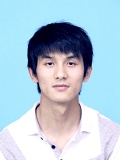
\includegraphics[width=0.2\textwidth\hfill]{xautjzd1.jpg}
\end{multicols}

%%% Education
%%% ------------------------------------------------------------
\NewPart{教育经历}{}

\EducationEntry{西安理工大学(硕士-保研)}{2012-至今}{软件工程}{研一研二期间作为实验室核心成员参与多个项目开发,并在研二课题研究中研究过Hadoop,最终转向行为识别与移动云计算迁移,比较熟悉常用的分类算法。}
\sepspace

\EducationEntry{西安理工大学(学士)}{2008-2012}{网络工程}{大一下自学C++;大二开始接触Linux,并开始钻研,Debian、Red Hat系列都玩过,最终选择Fedora;大二下自学Java,并研究过Struts2/Hibernate/Spring框架。}

%%% Skills
%%% ------------------------------------------------------------
\NewPart{个人技能}{}

\SkillsEntry{专业技能}{熟悉Ruby及Ruby on Rails}
\SkillsEntry{}{熟悉Vim, Git, Markdown}
\SkillsEntry{}{熟悉Linux C、Socket编程}
\SkillsEntry{}{熟悉Linux系统、Shell编程}
\SkillsEntry{}{熟悉机器学习常用算法,了解Hadoop}
\SkillsEntry{}{熟悉数据结构与与常用算法}
\SkillsEntry{}{熟悉HTML/JavaScript/Json/Ajax}
\SkillsEntry{}{熟悉ASP.NET MVC、SQL Server,了解MySQL、MongoDB}
\SkillsEntry{}{了解Java、Tex、函数式编程}
\SkillsEntry{英语水平}{CET-6}

%\SkillsEntry{Software}{\textsc{Matlab}, \LaTeX, \textsc{Ansys}, \textsc{Comsol}}

%%% Work experience
%%% ------------------------------------------------------------
\NewPart{项目经历}{}

\EducationEntry{远程医疗系统}{2014.1-2014.3}{}{此系统的框架主要由我负责完成。我主要负责将以前着手的几个项目各功能抽取出来,形成一个框架,同时将UI从以前的EasyUI转换到Bootstrap,并且在其中集成权限管理、基本增删改查、图表曲线显示、报表生成、地图显示及文件的上传与下载等常用功能。}
\sepspace

\EducationEntry{气调库环境监测系统}{2013.5-2013.11}{}{主要功能为数据转换及数据图表显示,由我单独完成。采集设备将采集到的数据存储在Access数据库中,由于某些原因,需要将Access中的数据导出来,并且以图表形式直观地展示各冷库参数,通过Web进行远程监控,而不用派专职人员蹲守在设备采集点。}
\sepspace

\EducationEntry{生产经营信息管理系统}{2012.8-2013.9}{}{主要功能为信息的录入及报表的生成。此系统由我和研三师兄两人负责设计开发,前期由我和师兄共同设计开发,后期由于师兄面临毕业,主要由我负责完成。}
\sepspace

\EducationEntry{果业技术服务平台}{2011.9-2012.6}{}{主要功能是信息的发布与信息的维护,分前后台,前台主要针对一般用户进行信息的浏览,而后台则由企业人员负责维护,进行信息的添加与发布。系统由我与师兄共同开发,前期师兄负责系统的设计,而我负责实现。}


%%% Awards & Honours
%%% ------------------------------------------------------------
\NewPart{获奖情况}{}

\HonorEntry{获得国家励志奖学金}{2009-2010}{}

\HonorEntry{获得院图灵杯科技节一等奖}{2010}{}

\HonorEntry{获得校三等奖学金}{2008-2009}{}

\HonorEntry{被评为2012届优秀毕业生}{2012}{}

\HonorEntry{被西安秦北学校评为优秀志愿者}{2013}{}

\HonorEntry{获得校三好学生荣誉称号}{2009-2010}{}

\HonorEntry{生产实习中与小组成员一起获得最具团队精神小组称号}{2011}{}

%%% Academic Honors
%%% ------------------------------------------------------------
\NewPart{研究成果}{}

\AcademicEntry{论文发表}{}{}{基于灰色系统理论的气调库环境预测模型[J]. 计算机系统应用,2014,23(3):123-126,118}
\sepspace

\AcademicEntry{软件著作权}{}{}{气调库环境监测系统,国家版权局,软件登记号:2014SR019840,2014.2.19}
\AcademicEntry{}{}{}{果品生产经营信息管理系统,国家版权局,软件登记号:2014SR039978,2014.04.09}
\sepspace

%%% Hobby
%%% ------------------------------------------------------------
%\NewPart{兴趣爱好}{}
%热爱打羽毛球、乒乓球,喜欢看网球比赛、读书,经常逛科技博客、GitHub、Hacker News和Startup News,时刻关注科技新闻和业界动态。

%%% Hobby
%%% ------------------------------------------------------------
\NewPart{自我评价}{}
热爱编程,喜欢钻研新语言、新技术,自学能力强,查找资料、分析解决问题能力强,同时敢于面对并克服困难,也能够吃苦耐劳,抗压能力较强。其次,我也一直很注重自己知识的储备,不断地给自己充电,养成每晚睡前阅读的习惯。
\end{CJK}     % 结束中文环境
\end{document}
